\subsection{MetaClust}
By clicking on the Toolset tab and then choosing MetaClust,
users are directed to the MetaClust homepage as in Figure~\ref{fig:metaClustHome}.
MetaClust \citep{huo2016meta} aims to perform sample clustering analysis combining multiple transcriptomic studies.
By integrating information from multiple studies of similar biological purposes,
MetaClust can identify a unified intrinsic gene set among all studies, perform weighted clustering analysis using the common intrinsic gene set, 
and match the clustering patterns across studies to define disease subtypes/cluster types.
The resulting clustering from meta-analysis is more robust and accurate than single study analysis.
The R package for the MetaClust module can be found at \url{https://github.com/metaOmics/MetaSparseKmeans}.


\begin{figure}[H]
\begin{center}
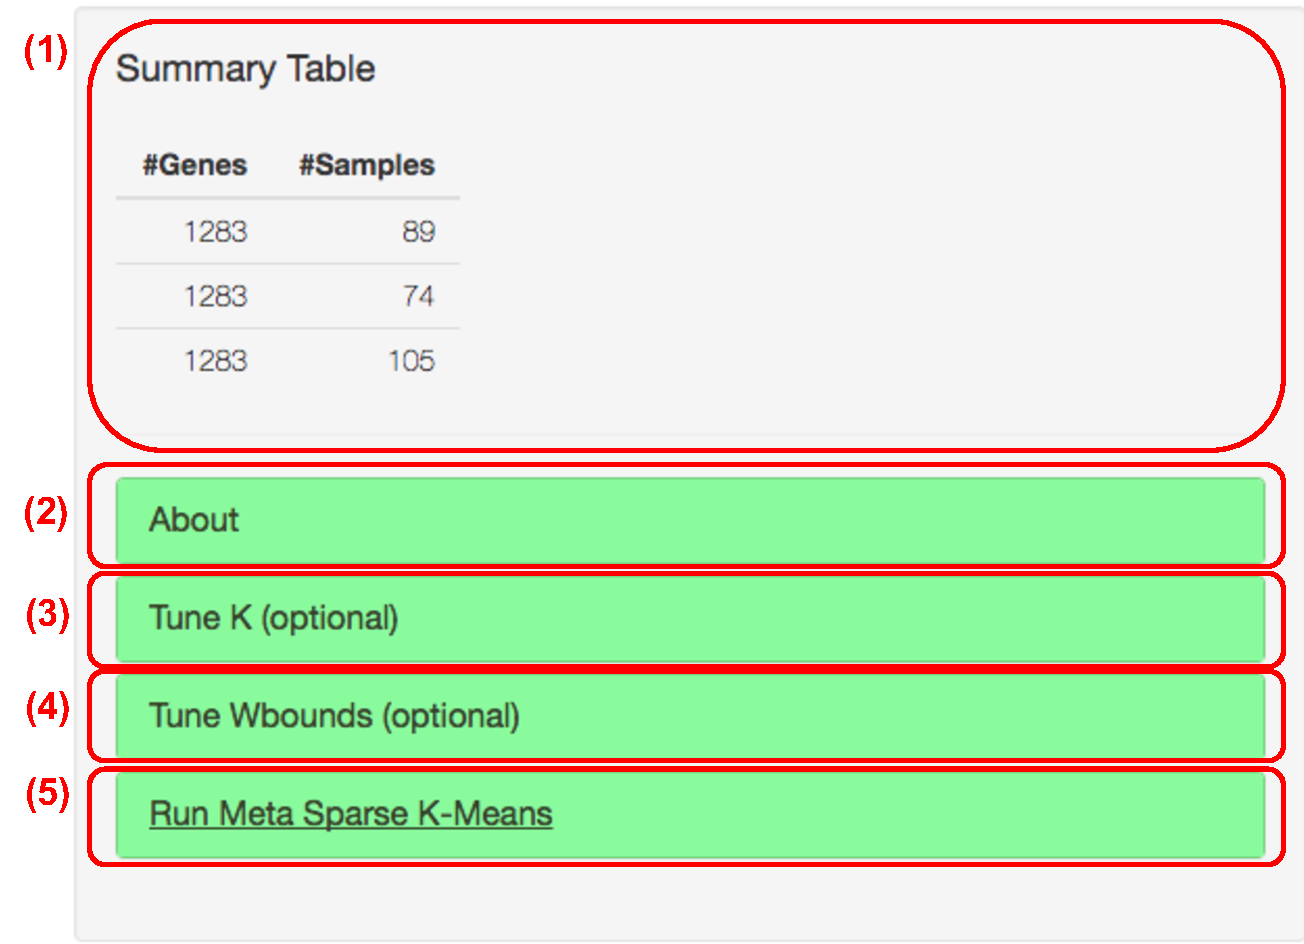
\includegraphics[scale=0.4]{./figure/metaClust/metaClustHome.pdf}
\caption{MetaClust homepage}
\label{fig:metaClustHome}
\end{center}
\end{figure}

\subsubsection{Procedure}


Figure~\ref{fig:metaClustHome} shows the homepage of MetaClust.
On the top-left panel, 
users can see the ``data summary table {\color{red} (1)}".
Below there are four tabs. 
``About tab {\color{red} (2)}"  describes basic introduction of MetaClust;
``Tune $K$ tab {\color{red} (3)}" performs tuning parameter selection for the number of clusters $K$;
``Tune Wbounds tab {\color{red} (4)}" performs tuning parameter selection for the number of selected features, where a larger Wbound will yield more selected genes;
``Run Meta Sparse $K$-Means tab {\color{red} (5)}" performs the MetaClust algorithm.
Starting with multiple studies, 
we could run MetaSparseKmeans {\color{red} (5)} with pre-specified number of clusters ($K$) and gene selection tuning parameter (Wbounds).
If you are not sure about what constitutes good $K$ and Wbounds, 
users are advised to use the ``Tune $K$ {\color{red} (3)}" and ``Tune Wbounds {\color{red} (4)}" panel.
A complete list of options is available in Section~\ref{sec:completeList_MetaClust}.

\begin{steps}

\item \textbf{Tune $K$:} 

\begin{figure}[H]
\begin{center}
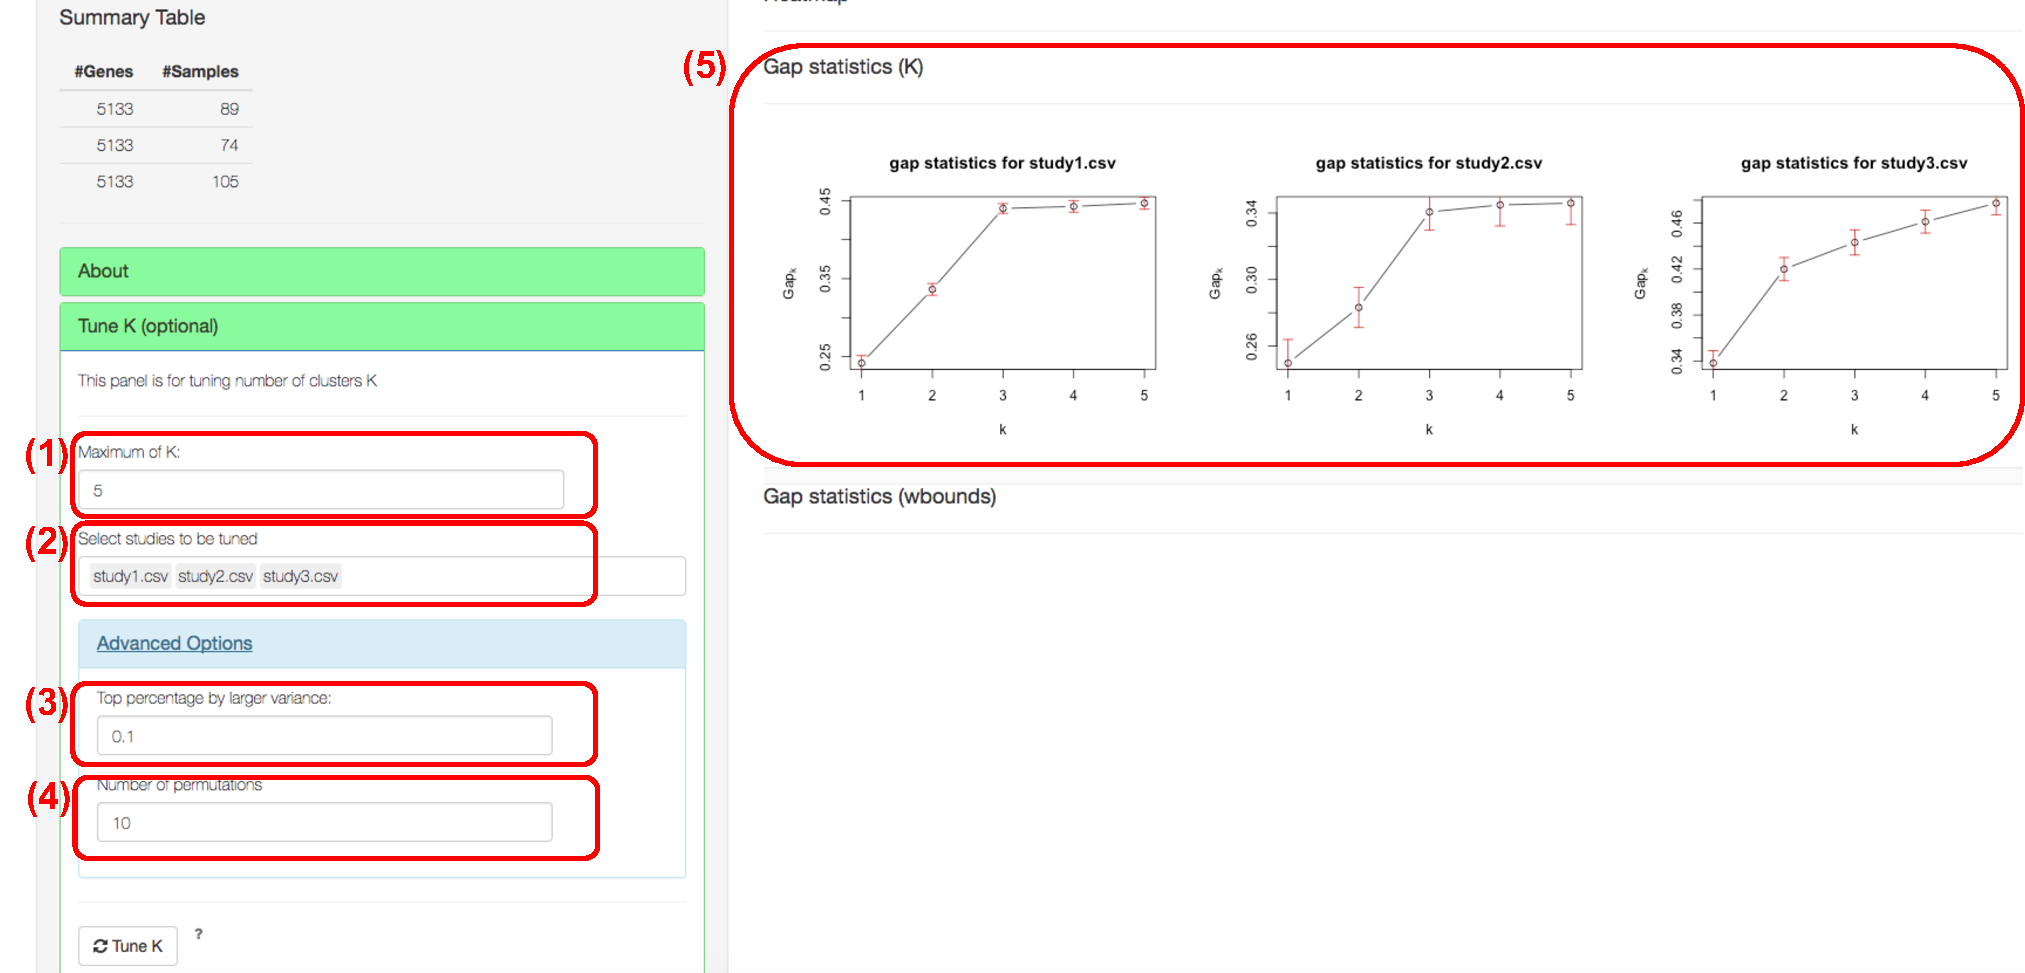
\includegraphics[scale=0.5]{./figure/metaClust/tuneK.pdf}
\caption{Tuning parameter selection for number of clusters.
A good $K$ is selected such that the $\mbox{Gap}_k$ is maximized or stabilized across all studies.
}
\label{fig:metaClusttuneK}
\end{center}
\end{figure}

If the users are not sure what is the number of clusters,
they can start to use the ``Tune $K$ panel" as in Figure~\ref{fig:metaClusttuneK}.
Gap statistics will be used to get optimal $K$ for each individual study.
Detailed descriptions of the gap statistics can be found \cite{tibshirani2001estimating}.
Users need to specify the maximum number of $K$ {\color{red} (1)}, 
with which the algorithm will search number of studies from 1 to $K$.
Studies to be tuned can be selected {\color{red} (4)}.
In advanced options, users can further specify the number of top variance genes to be included and number of permutations.
But if users don't know the algorithm, please leave them as default.
Top percentage p\% by larger variance means that we will use top p\% larger variance genes to perform gap statistics {\color{red} (3)}.
The number of permutations is the number of bootstrap samples for gap statistics {\color{red} (4)}.
At least 50 bootstrap samples are suggested for a stable result of number of clusters.
By clicking the button ``Tune $K$,"
users will obtain the gap statistics, 
as in Figure~\ref{fig:metaClusttuneK}.
A good $K$ is selected such that the $\mbox{Gap}_k$ is maximized or stabilized across all studies.
From the figure, $K=3$ is preferred since the gap statistics from all three studies become flat {\color{red} (5)}.

\item \textbf{Tune Wbounds:} 

Wbounds directly control number of features selected by the MetaClust module.
A larger number of Wbounds will result in more numbers of selected genes.
If the users are not sure what is a good Wbound,
they can start to use the ``Tune Wbounds panel", 
as in Figure~\ref{fig:metaClusttuneW}.
\begin{figure}[H]
\begin{center}
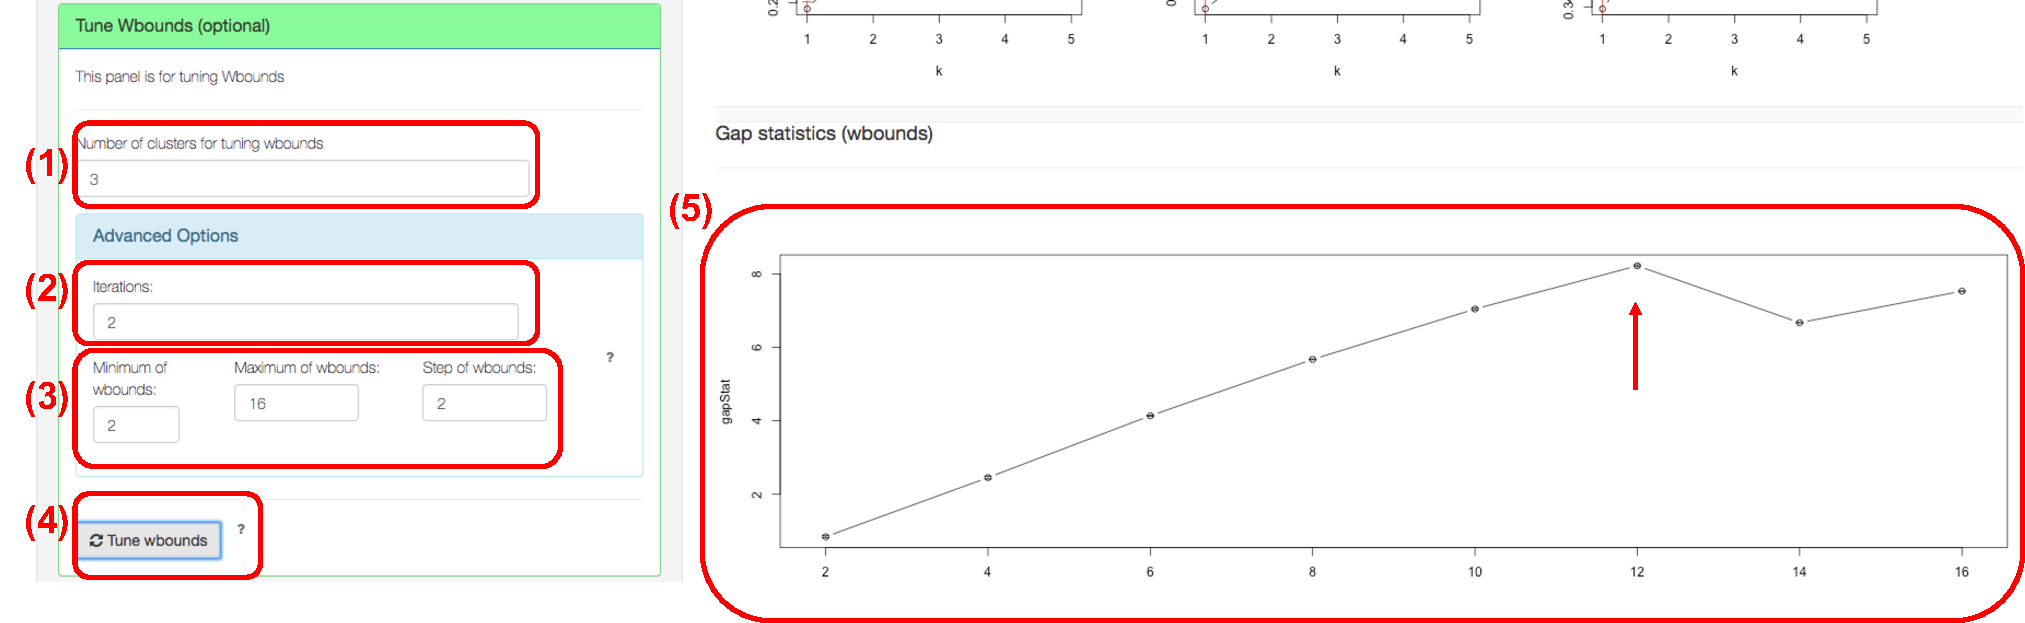
\includegraphics[scale=0.5]{./figure/metaClust/tuneW.pdf}
\caption{Wbound selection.
The Wbound controls the number of selected features.
A larger Wbound will yield a larger number of selected genes.
The optimum Wbound is selected when the gap statistics is maximized.
}
\label{fig:metaClusttuneW}
\end{center}
\end{figure}
Again,
gap statistics will be used for tuning Wbounds.
Users will specify the number of clusters for tuning Wbounds {\color{red} (1)}, which could be obtained from the previous step.
In advanced options, users can further specify the number of iterations and the range of candidate Wbounds.
But if users don't know the algorithm, please leave them as default.
Iterations {\color{red} (2)} specify the number of bootstrap samples for gap statistics.
Users also need to specify the searching space of Wbounds by minimum of Wbounds, maximum of Wbounds, and step of Wbounds {\color{red} (3)}.
After all these steps are set,
the user can click on the ``Tune Wbounds" button {\color{red} (4)}.
The results will be shown in Figure~\ref{fig:metaClusttuneW} {\color{red} (5)}.
Wbound=12 is preferred since the corresponding gap statistics is maximized (where the red arrow indicates).

\item \textbf{Run MetaClust:} 

Under the ``Run Meta Sparse K-Means" panel,
the user can specify the number of clusters {\color{red} (1)} and Wbounds {\color{red} (2)}, and run MetaClust {\color{red} (5)}, 
as in Figure~\ref{fig:mskmRes}.
\begin{figure}[H]
\begin{center}
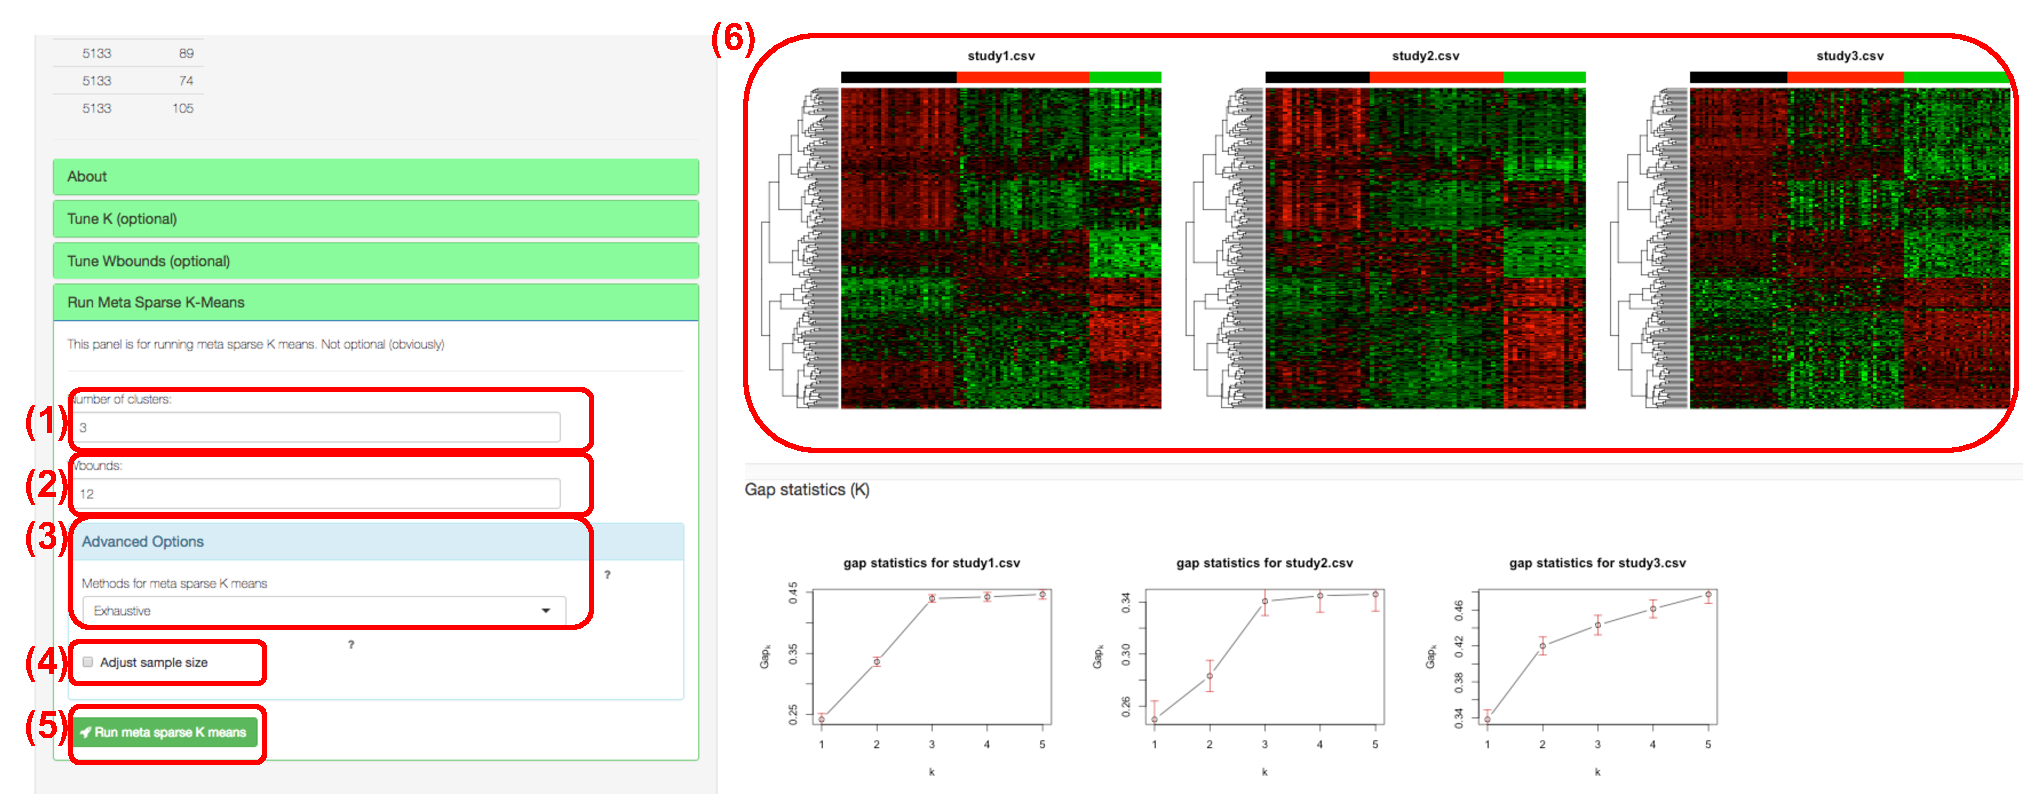
\includegraphics[scale=0.5]{./figure/metaClust/mskmRes.pdf}
\caption{Result for MetaClust.
The heatmap on top shows the gene-expression profiles of the three studies with selected features.
Each row represents a gene, and each column represents a sample.
Note that the three studies share a common set of genes.
The color bar on top of the heatmap represents the subtype labels.
For instance, the black bar on top of each study represents the same subtype  for all studies.
Clearly, we could see distinct subtype patterns, and these patterns are consistent across studies.
}
\label{fig:mskmRes}
\end{center}
\end{figure}
In advanced options (which users are not adviced to change if they are not familiar with the algorithm), 
there are three clustering matching methods {\color{red} (3)}: exhaustive, linear, and MCMC.
Exhaustive is suggested if the data is not large.
Currently, only the exhaustive search method is implemented.
``Adjust sample size" checkbox (at position {\color{red} (5)}) allows users to adjust sample size effect.
After the number of clusters and Wbounds are specified,
users can click on the ``Run meta sparse $K$ means" and obtain results, 
as shown in Figure~\ref{fig:mskmRes}.
\end{steps}


\subsubsection{Results}

We used the leukemia data to demonstrate the MetaClust module.
After merging the three datasets, we didn't filter out any genes (filter 0\% genes by mean and 0\% by variance); 
thus 5133 genes remained.
Detailed descriptions of these studies can be found in Table~\ref{tab:realDataLeukemia}. 
In this example, we do not need the extra label information.
The result is shown in Figure~\ref{fig:mskmRes} {\color{red} (5)}.
We obtained unified feature selection across all studies.
The clusters are well separated in each study, and the cluster patterns are consistent across all studies.
The clustering heatmaps and labels are saved in the MetaClust folder.










